\begin{frame}{Konstrukcija pravokotnice}
\begin{columns}[T,onlytextwidth]

\begin{column}{0.55\textwidth}
\small
\begin{itemize}
    \item<1-> Dana sta premica \(p\) in točka \(T\).
    \item<2-> Nariši lok \(l_1\) s središčem v \(T\).
    \item<3-> Lok \(l_1\) seka premico \(p\) v točkah \(A\) in \(B\).
    \item<4-> Nariši lok \(l_2\) s središčem v \(A\).
    \item<5-> Nariši lok \(l_3\) s središčem v \(B\) in z enakim polmerom.
    \item<6-> Loka se sečeta v točki \(C\).
    \item<7-> Premica \(TC\) je pravokotna na \(p\).
\end{itemize}
\end{column}

\begin{column}{0.45\textwidth}
\centering
\only<1>{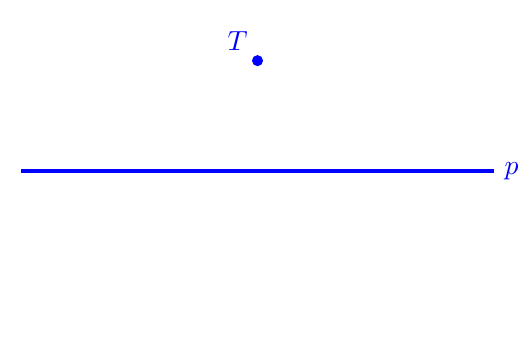
\includegraphics[width=\linewidth,keepaspectratio]{slike/fig-1.png}}
\only<2>{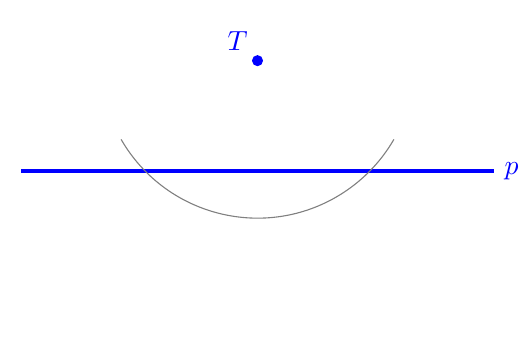
\includegraphics[width=\linewidth,keepaspectratio]{slike/fig-2.png}}
\only<3>{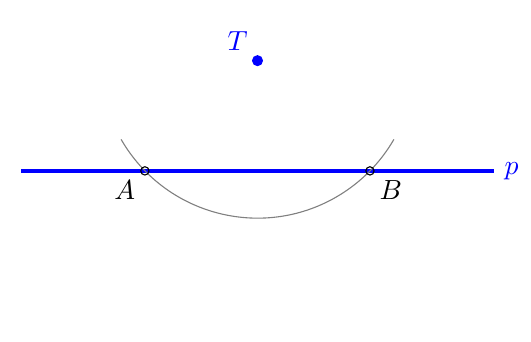
\includegraphics[width=\linewidth,keepaspectratio]{slike/fig-3.png}}
\only<4>{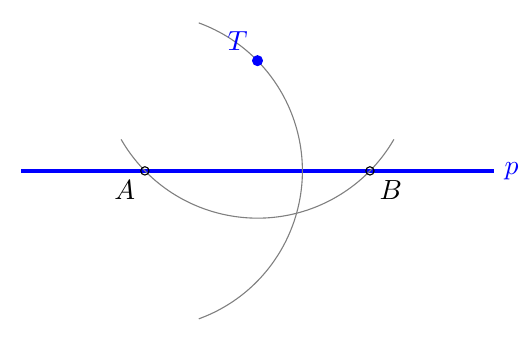
\includegraphics[width=\linewidth,keepaspectratio]{slike/fig-4.png}}
\only<5>{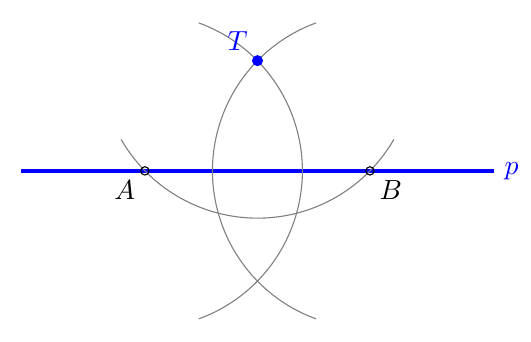
\includegraphics[width=\linewidth,keepaspectratio]{slike/fig-5.png}}
\only<6>{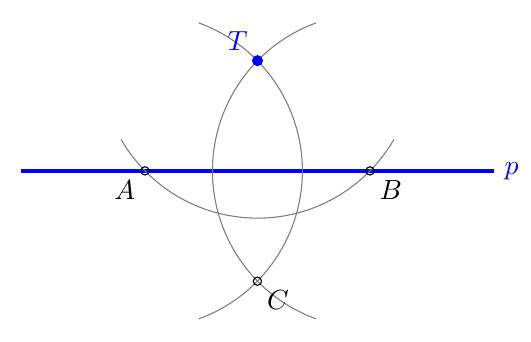
\includegraphics[width=\linewidth,keepaspectratio]{slike/fig-6.png}}
\only<7>{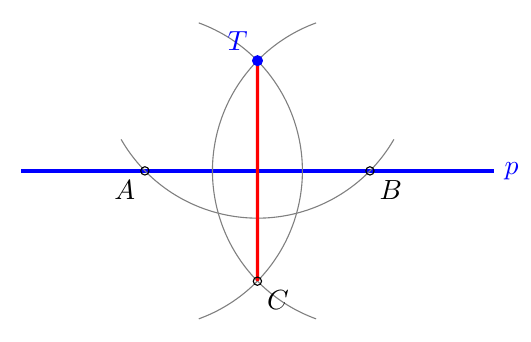
\includegraphics[width=\linewidth,keepaspectratio]{slike/fig-7.png}}
\end{column}

\end{columns}
\end{frame}